% -----------------------------------------------
% Vlastní text práce (kapitoly práce)
% -----------------------------------------------

% -----------------------------------------------
\chapter{Calibration UV optical source}
% -----------------------------------------------
Blah blah we need it.
% -----------------------------------------------
\section{Karlsruhe UV source}
% -----------------------------------------------

% -----------------------------------------------

\section{Testing and measurement of UV source}
% -----------------------------------------------
For calibration UV source, the longtime stability of optical power and pulse geometry is very important. Because there were no specialized apparatus for this measurement, we had to built and program one by ourselves.
\subsection{Measuring apparatus}
For measuring the optical power we use PM16 power meter (PM) and for determining the pulse geometry we use XP2262 PMT with signal output connected to 2-channel PicoScope 2205A MSO usb osciloscope.
\par
We also use DS18B20 thermometer for PMT temperature monitoring and keysight 34461a multimeter for checking voltages.

\par
The PMT, power meter and the optical head of UV source are mounted in the IS's ports. The IS stops the unwanted external light and distributes the optical power to PMT and power meter. 
\par
The entire apparatus is driven by Raspberry Pi (RPi). The RPi takes care of data acquisiton and could be used to set the parameters of UV source. It could be easilly accessed over internet for data download or for user to control the experiment.
\par


\par
The apparatus could be seen on fig. \ref{aparature1} and \ref{aparature2}.

\begin{figure}[H]
 \centering
 \includegraphics[width=150mm]{./pictures/aprature1b}
 \caption{Measuring apparatus.}
 \label{aparature1}
\end{figure}

\begin{figure}[H]
 \centering
 \includegraphics[scale = 0.09]{./pictures/aparature2b}
 \caption{PMT mounting and HV source.}
 \label{aparature2}
\end{figure}


\subsection{Data acquisition and analysis}
All the data are taken in specified interval (15 or 30 minutes). Two files are produced - osciloscope waveform file and a file with 30 samples of power meter, multimeter and a thermometer readings.
\par
The data from osciloscope contains the square pulses with noise (fig. \ref{pulse}). From them we need to extract the information of pulses height, slope and time of the rising edge.

 \begin{figure}[H]
 \centering
 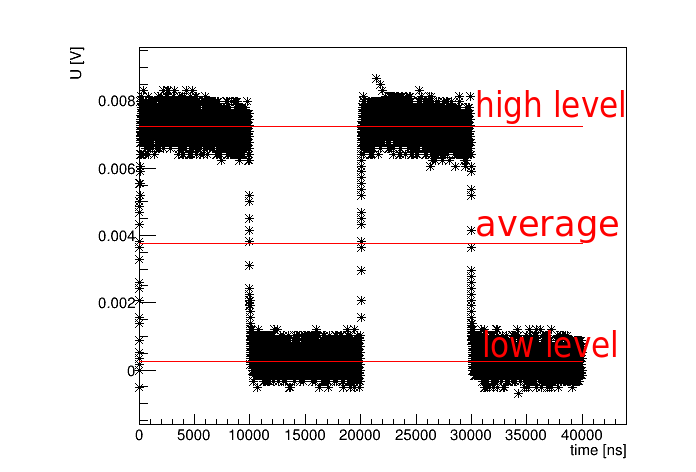
\includegraphics[scale=0.65]{./pictures/PMTPulse}
 \caption{Determining the pulse properties from average, low and high levels of signal.}
 \label{pulse}
\end{figure}



\subsection{Results}

\section{UV LED diode aging}

%------------------------------------------------
\section{Optical feedback - potential fix}
% -----------------------------------------------
One way to handle the aging process of UV LED diodes is to monitor the power and according to the changes set the diode current. 


%------------------------------------------------

\section{Modified UV source for drone mounting}
% -----------------------------------------------



% -----------------------------------------------
% %%%%%%%%%%%%%%%%%%%%%%%% End of file %%%%%%%%%%%%%%%%%%%%%%%%
